% feasibility-report.tex: 可行性报告
% Copyright (C) 2022 吴骏东, 张子辰, 蓝俊玮, 郭耸霄 and 陈建绿
% All rights reserved.

% This file is part of Runikraft. Runikraft is free software,
% which is released under the BSD 3-Clause License, see LICENSE for details.
% Runikraft is provided ``as is'', without any express or implied warrenties.

% The reports of Runikraft are released under the Creative Commons
% Attribution 4.0 International License; see report/LICENSE for details.
\documentclass[UTF8,fontset=none,linespread=1.15]{ctexart}
\ctexset
{
    section/format={\Large\sffamily\bfseries},
    subsection/format+={\sffamily},
    subsubsection/format+={\itshape}
}
\setCJKmainfont[ItalicFont={KaiTi},BoldItalicFont={KaiTi},
BoldItalicFeatures={FakeBold=3}]{Noto Serif CJK SC}
\setCJKsansfont[BoldFont={Noto Sans CJK SC Bold},
BoldItalicFont={Noto Sans CJK SC Bold},
AutoFakeSlant]{Noto Sans CJK SC DemiLight}
\setCJKmonofont[AutoFakeBold=3,AutoFakeSlant]{FangSong}
\setmainfont{cmun}[Extension=.otf,UprightFont=*rm,
ItalicFont=*ti,BoldFont=*bx,BoldItalicFont=*bi]
\setsansfont{cmun}[Extension=.otf,UprightFont=*ss,
ItalicFont=*si,BoldFont=*sx,BoldItalicFont=*so]
\setmonofont{cmun}[Extension=.otf,UprightFont=*btl,
ItalicFont=*bto,BoldFont=*tb,BoldItalicFont=*tx]
%Computer Modern Unicode 的\textasciitilde和\~{}的高度相同,所以用\tildechar表示居中的波浪线~
\newcommand{\tildechar}{\raisebox{-0.35em}{\textasciitilde}}
\usepackage[a4paper,hmargin=1.2in,vmargin=1in]{geometry}
\usepackage{graphicx,tikz,float,multicol,makecell,multirow,longtable}
\usepackage{verbatim}
\usepackage[normalem]{ulem}
\usepackage{CJKfntef}
\usepackage[perpage]{footmisc}

%目录, 参考了OSH-2021/x-sBPF
\usepackage{titletoc}
\titlecontents{section}[2em]{\addvspace{1.3mm}\bfseries}{%
\contentslabel{2.0em}}{}{\titlerule*[5pt]{$\cdot$}\contentspage}
\titlecontents{subsection}[4.2em]{}{\contentslabel{2.5em}}{}{%
\titlerule*[5pt]{$\cdot$}\contentspage}
\titlecontents{subsubsection}[7.2em]{}{\contentslabel{3.3em}}{}{%
\titlerule*[5pt]{$\cdot$}\contentspage}

%图表标题
\usepackage{caption}
\captionsetup{font={sf}}

%代码环境
\usepackage{listings}
\lstset{basicstyle={\normalfont\ttfamily},breaklines,tabsize=4}
\renewcommand{\lstlistingname}{代码}
\renewcommand{\lstlistlistingname}{代码}
%Rust
\lstdefinelanguage{Rust}
{
    morekeywords={as,async,await,break,const,continue,crate,dyn,else,enum,extern,false,fn,for,if,impl,in,let,loop,match,mod,move,mut,pub,ref,return,Self,self,static,struct,super,trait,true,type,union,unsafe,use,where,while,abstract,become,box,do,final,macro,override,priv,try,typeof,unsized,virtual,yield},
    sensitive=true,
    morecomment=[l]{//},
    morecomment=[s]{/*}{*/},
    morestring=[b]{"},
    morestring=[b]{'}
}


\usepackage{enumitem}
\setlistdepth{5}
\renewlist{enumerate}{enumerate}{5}
\setlist{itemsep=0pt,partopsep=0pt,parsep=0pt,topsep=0pt}
\setlist[enumerate,1]{label=\arabic*.}
\setlist[enumerate,2]{label=(\arabic*)}
\setlist[enumerate,3]{label=\textcircled{\arabic*}}
\setlist[enumerate,4]{label=(\textit{\roman*})}
\setlist[enumerate,5]{label=\textit{\alph*})}

\usepackage[colorlinks,unicode,pdfstartview={FitH}]{hyperref}
\hypersetup
{
  pdftitle={2022春 操作系统原理与设计(H) x-runikraft小组 可行性报告},
  pdfauthor={吴骏东; 张子辰; 蓝俊玮; 郭耸霄; 陈建绿}
}

%带圈数字,它必须在hyperref之后载入
\usepackage{xunicode-addon}
\makeatletter
\xeCJKDeclareCharClass{CJK}{"24EA, "2460->"2473, "3251->"32BF,"24B6->"24E9,"2160->"217F}
\newfontfamily\EnclosedNumbers{Noto Serif CJK SC}
\AtBeginUTFCommand[\textcircled]{\begingroup\EnclosedNumbers}
\AtEndUTFCommand[\textcircled]{\endgroup}
\makeatother

\makeatletter
\let\textcircled@old\textcircled
\protected\def\textcircled#1{%
	\expandafter\textcircled@old\expandafter{\expanded{#1}}}
\makeatother
\makeatletter
\renewcommand\@makefntext[1]{%
	\setlength\parindent{0.75\ccwd}\selectfont
	\@thefnmark\ #1}
\makeatother
\renewcommand*\thefootnote{\textcircled{\arabic{footnote}}}
\renewcommand{\lstlistingname}{代码}

%上标+引用
\let\nosupcite\cite
\renewcommand*{\cite}[1]{\textsuperscript{\nosupcite{#1}}}

%章节作者
\newcommand{\sectionauthor}[1]{%
\vspace*{-5ex}
\noindent\textrm{\hfill\textit{by #1}}
\vspace*{2ex}\par}
%\renewcommand{\today}{2022年4月5日}

\begin{document}
\sffamily %为方便屏幕阅读,文档主要使用无衬线字体
\title{\bfseries Runikraft小组\quad 可行性报告}
\author{吴骏东\and 张子辰\and 蓝俊玮\and 郭耸霄\and 陈建绿}
\date{\today}
\maketitle

\tableofcontents

\section{理论依据}
\subsection{Rust Language}

A language empowering everyone to build reliable and efficient software.

\subsubsection{Advantages}
\paragraph{Performance}Rust is blazingly fast and memory-efficient: with no runtime or garbage collector, it can power performance-critical services, run on embedded devices, and easily integrate with other languages.

\paragraph{Reliability}Rust’s rich type system and ownership model guarantee memory-safety and thread-safety — enabling you to eliminate many classes of bugs at compile-time.

\paragraph{Productivity}Rust has great documentation, a friendly compiler with useful error messages, and top-notch tooling — an integrated package manager and build tool, smart multi-editor support with auto-completion and type inspections, an auto-formatter, and more.

\subsubsection{Applications}

用Rust改写项目已经成为一种解决问题的有效手段,如zalando公司从Scala转向Rust的成功故事。\cite{3}

\subsection{RISC-V Architecture}

RISC-V is a free and open ISA enabling a new era of processor innovation through open standard collaboration.

The RISC-V ISA delivers a new level of free, extensible software and hardware freedom on architecture, paving the way for the next 50 years of computing design and innovation.

\subsubsection{Advantages}

1. RISC(精简指令集计算)架构具有一组指令,因此高级语言编译器可以生成更有效的代码。
2. 由于其简单性,它允许自由使用微处理器上的空间。
3. 许多RISC处理器使用寄存器来传递参数和保存局部变量。
4. RISC函数仅使用几个参数,而RISC处理器无法使用调用指令,因此,使用易于流水线化的固定长度指令。
5. 操作速度可以最大化,执行时间可以最小化。
6. 所需的指令格式数量很少,所需的指令数量和寻址方式也很少。\cite{4}

\subsubsection{Applications}

目前基于RISC-V架构的开源处理器有很多,既有标量处理器Rocket,也有超标量处理器BOOM,还有面向嵌入式领域的Z-scale、PicoRV32等。\cite{2}

\subsection{QEMU}

QEMU is a generic and open source machine emulator and virtualizer.

When used as a machine emulator, QEMU can run OSes and programs made for one machine (e.g. an ARM board) on a different machine (e.g. your own PC). By using dynamic translation, it achieves very good performance.

When used as a virtualizer, QEMU achieves near native performance by executing the guest code directly on the host CPU. QEMU supports virtualization when executing under the Xen hypervisor or using the KVM kernel module in Linux. When using KVM, QEMU can virtualize x86, server and embedded PowerPC, 64-bit POWER, S390, 32-bit and 64-bit ARM, and MIPS guests.\cite{1}

\subsubsection{Advantages}

\paragraph{Full-system emulation}Run operating systems for any machine, on any supported architecture.

\paragraph{User-mode emulation}Run programs for another Linux/BSD target, on any supported architecture.

\paragraph{Virtualization}Run KVM and Xen virtual machines with near native performance.\cite{1}


\section{技术依据}
\section{创新点}
\section{概要设计}
Runikraft的架构与Unikraft几乎相同。
\begin{figure}[!hbt]
\centering
\begin{minipage}{0.49\linewidth}
\centering
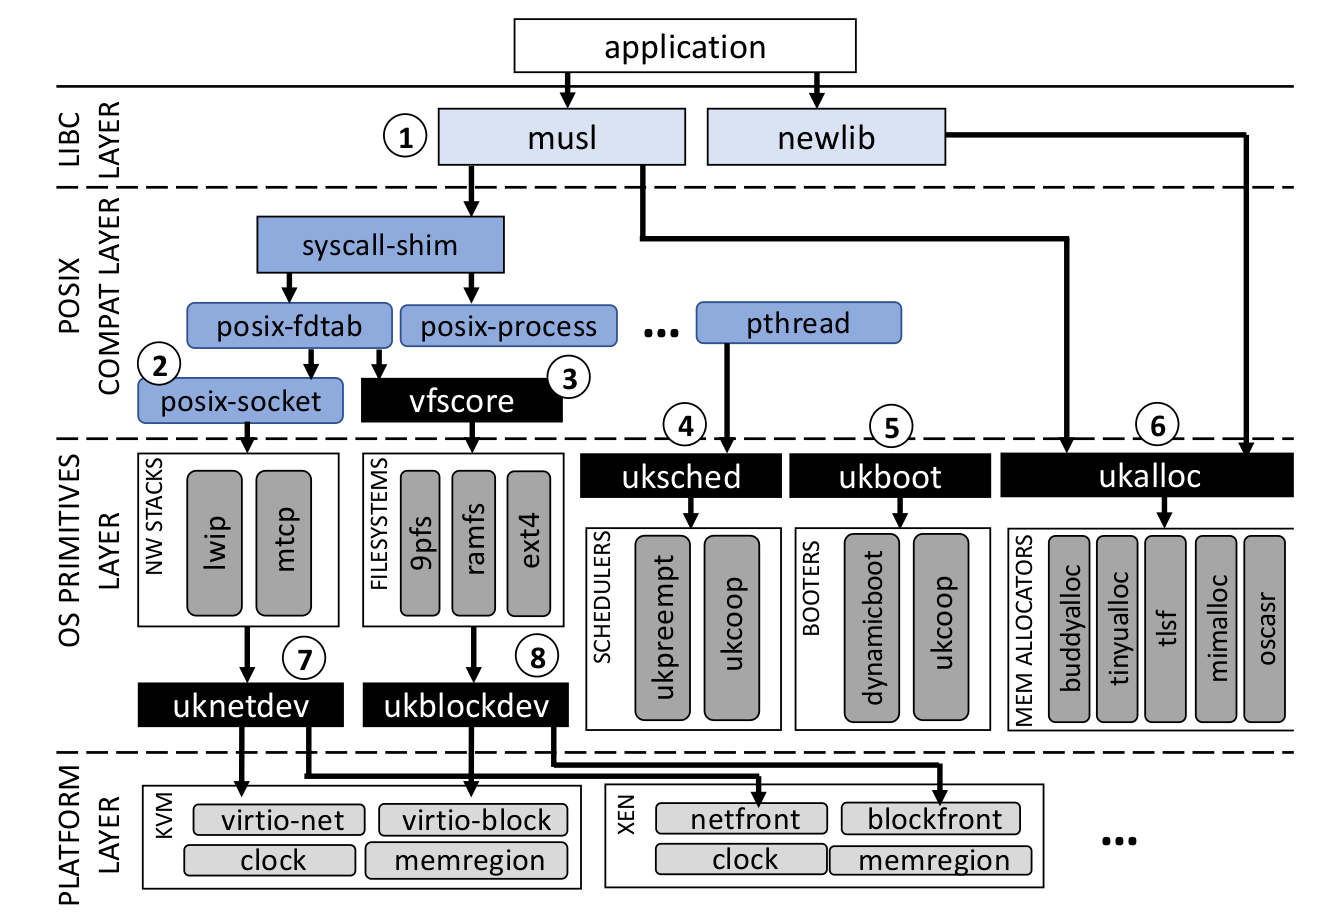
\includegraphics[width=\linewidth]{assets/Unikraft-architecture.png}
\caption{Unikraft的架构}\label{fig:unikraft-arch}
\end{minipage}
\begin{minipage}{0.49\linewidth}
\centering
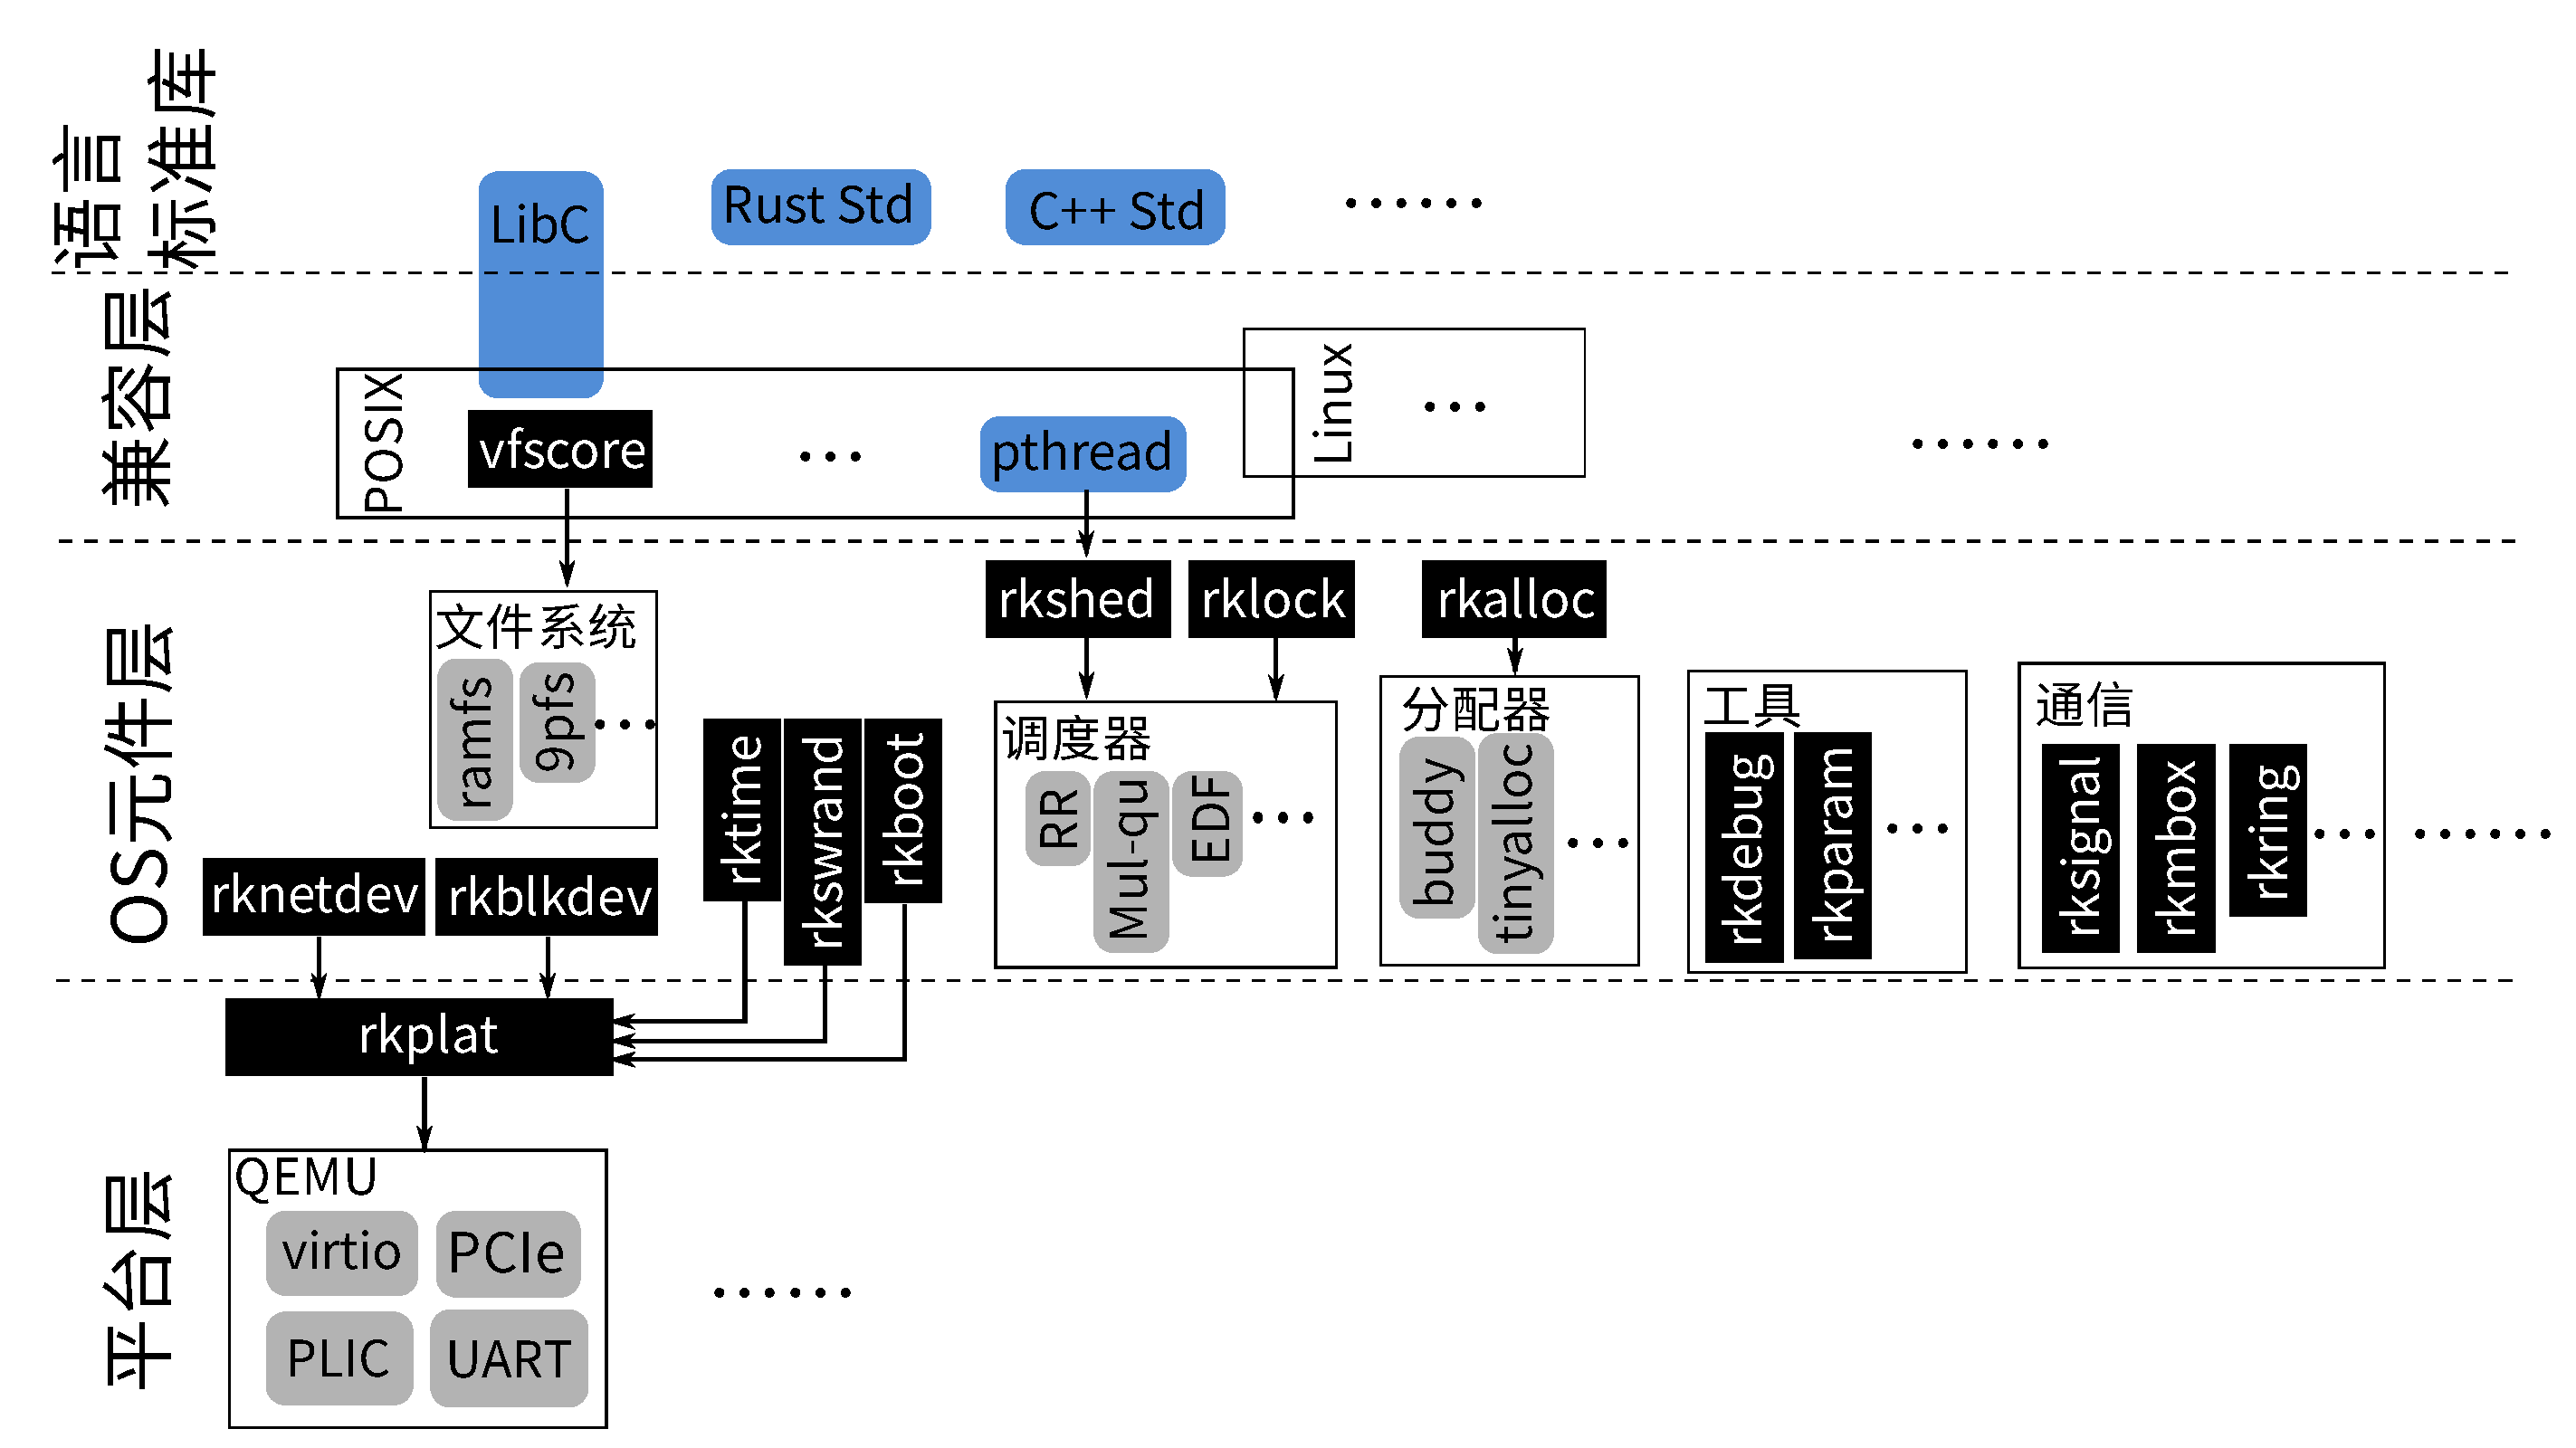
\includegraphics[width=\linewidth]{assets/Runikraft-architecture.pdf}
\caption{Runikraft的架构}\label{fig:runikraft-arch}
\end{minipage}
\end{figure}
平台层将不同的平台封装成通用的\texttt{rkplat} API,它提供与平台/架构密切相关的功能,
比如外设驱动、外中断处理、内存分页、定时器、原子操作、内存屏障,我们只计划支持RISC-V+QEMU virt
一种平台。如果时间不足,我们可以将现成的OpenSBI\cite{5}\cite{6}封装成\texttt{rkplat} API。

\texttt{rknetdev}、\texttt{rkblkdev}、\texttt{rktime}、\texttt{rkswrand}、\texttt{rkboot}
五个APIs的功能与平台密切相关,
但是为了降低开发和维护难度,它们并没有直接实现,而是在\texttt{rkplat}提供的初级抽象的基础上实现。
\texttt{rknetdev}和\texttt{rbblkdev}对应图\ \ref{fig:un{}ikraft-arch}\ 的⑦和⑧,
它们分别提供网络设备和块设备的支持。
%与Unikraft的实现类似,这两个APIs的构造函数的参数接受指向\texttt{trait RKplat}的指针。
\texttt{rktime}提供获取和修改系统时间的API,\texttt{rkswrand}提供密码学安全的随机数,
\texttt{rkboot}负责完成系统的初始化并将控制权转交给用户的代码。

\texttt{rkshed}和\texttt{rklock}是两个与调度器有关的APIs,前者负责创建、调度、撤销线程,后者负责线程间
的同步和互斥。Runikraft支持多种调取器,比如,图\ \ref{fig:runikraft-arch}\ 中的RR的时间片轮转调度器、
Mul-qu是多重队列调取器、EDF是截止日期有限调度器。我们计划先实现RR调度器。当然,为了系统镜像的轻量性,
用户可以不使用任何调取器,这时,\texttt{rkshed}和\texttt{rklock}会被编译成空API,创建线程的行为
将和函数调用相同。这保证了大部分使用仅仅并行加速的程序仍然能正确运行。

Runikraft选择性地提供线程通信模块,如UNIX风格的信号(\texttt{rksignal}),信箱(\texttt{rkmbox}),
无锁的环形缓冲队列(\texttt{rkring})。

我们目前没有计划区分线程和进程,Runikraft的线程同时具有传统的OSes的线程和进程的特性:
线程之间没有隔离措施,但是线程之间又可以使用进程通信的方法更安全地同步。

\texttt{rkalloc}是分配器API,它的后端可以是\texttt{buddy}、\texttt{tinyalloc}、\texttt{tlsf}、
\texttt{mimalloc}等分配器。
不过,我们可能只会实现其中的一个。

Runikraft还提供了一些工具模块,比如调试工具\texttt{rkdebug}、命令行参数分析工具\texttt{rkparam}。

在 Unikraft 中,文件系统 API vfscore 是 POSIX 兼容层的一部分,我们沿用了它的设
计,将 \texttt{vfscore} 放在了兼容层。Runikraft计划支持RAM上的临时文件系统和Plan 9 OS的9fps。

位于最顶层的是语言标准库,这一层可以帮助Runikraft支持多种语言。
虽然语言标准库层被画在了兼容层之上,但它其实是直接用OS元件层的APIs实现的,这能避免分层系统
的低效。
我们只打算实现Rust标准库和C标准库的部分内容。


\section*{许可协议}
本文档以知识共享署名 4.0 国际 (CC BY 4.0)许可证发布。

\vspace{2ex}
\noindent\textbf{\large 您可以自由地}:
\begin{description}
\item[共享] 在任何媒介以任何形式复制、发行本作品;
\item[演绎] 修改、转换或以本作品为基础进行创作
在任何用途下,甚至商业目的。
\end{description}

\vspace{2ex}
\noindent\textbf{\large 惟须遵守下列条件}:
\begin{description}
\item[署名] 您必须给出适当的署名,提供指向本许可协议的链接,
同时标明是否(对原始作品)作了修改。您可以用任何合理的方式来署名,
但是不得以任何方式暗示许可人为您或您的使用背书。
\item[没有附加限制] 您不得使用法律术语或者技术措施,从而限制其他人
做许可协议允许的事情。
\end{description}

\vspace{2ex}
\noindent\textbf{\large 声明}:

您不必因为公共领域的作品要素而遵守许可协议,或者您的使用被可适用的例外或限制所允许。

不提供担保。许可协议可能不会给与您意图使用的所必须的所有许可。
例如,其他权利比如形象权、隐私权或人格权可能限制您如何使用作品。

本许可证的全文位于:\\
\centerline{\url{https://creativecommons.org/licenses/by/4.0/legalcode.zh-Hans}}
\bibliographystyle{IEEEtran}
\bibliography{feasibility-report}
\end{document}